\documentclass[a4paper,11pt]{scrartcl}

\usepackage[utf8]{inputenc}
\usepackage[T1]{fontenc}
\usepackage{amsmath,amsthm,amssymb}
\usepackage{lmodern}
\usepackage{xspace}
\usepackage[french]{babel}
\usepackage{graphicx}
\usepackage[section]{placeins}
\usepackage{braket}
\usepackage{listings}
\usepackage{xcolor}
\usepackage{tikz}
\usepackage[hidelinks]{hyperref}
\usepackage{fancyhdr}

\pagestyle{fancy}
\fancyhf{}
\renewcommand{\headrulewidth}{2pt}
\renewcommand{\footrulewidth}{1pt}
\lhead{\leftmark}
\cfoot{\thepage}
%\rfoot{\rightmark}
%\lfoot{BENJELLOUN Youssef}

% definitions des theoremes
\theoremstyle{plain}
\newtheorem{thm}{Théorème}[section]
\newtheorem{prop}[thm]{Proposition}
\newtheorem{lemme}[thm]{Lemme}
\theoremstyle{definition}
\newtheorem{defi}[thm]{Définition}
\newtheorem{exo}{Exercice}[section]

\def\checkmark{\tikz\fill[scale=0.4](0,.35) -- (.25,0) -- (1,.7) -- (.25,.15) -- cycle;}

\lstdefinestyle{myStyle}{
    belowcaptionskip=1\baselineskip,
    breaklines=true,
    frame=none,
    numbers=none,
    basicstyle=\footnotesize\ttfamily,
    keywordstyle=\bfseries\color{green!40!black},
    commentstyle=\itshape\color{purple!40!black},
    identifierstyle=\color{blue},
    backgroundcolor=\color{gray!10!white},
}
% Style emprunté de https://nasa.github.io/nasa-latex-docs/html/examples/listing.html



% commandes personnelle\s
\newcommand{\ensemble}[1]{\mathbb{#1}}
\newcommand{\R}{\ensemble{R}}
\newcommand{\dijkstra}{\nom{Dijkstra}}
\newcommand{\nom}[1]{\bsc{#1}\xspace}
\newcommand{\algo}{algorithme de \dijkstra}
\newcommand{\glms}[1]{\og#1\fg}

% Définitions pour le titre du document
\title{L'algorithme de Dijkstra en partant de zéro}
\author{Youssef Benjelloun}

\begin{document}
\maketitle
\tableofcontents

\section*{Introduction}
En théorie des graphes, l'\algo sert à résoudre le problème du plus court
chemin. Il permet, par exemple, de déterminer un plus court chemin pour se
rendre d'une ville à une autre connaissant le réseau routier d'une région.
Plus précisément, il calcule des plus courts chemins à partir d'une source
vers tous les autres sommets dans un graphe orienté pondéré par des réels
positifs. On peut aussi l'utiliser pour calculer un plus court chemin entre
un sommet de départ et un sommet d'arrivée.
\section{Biographie}
Edsger Wybe \dijkstra né à Rotterdam le 11 mai 1930 et mort Nuenen le
6 août 2002, est un mathématicien et informaticien néerlandais du
\textsc{xx}\ieme siécle. Il reçoit en 1972 le prix Turing pour ses
contributions sur la science et l’art des langages de programmation et au
langage Algol. Juste avant sa mort, en 2002, il reçoit le prix PoDC de
l'article influent, pour ses travaux sur l'autostabilisation. L'année
suivant sa mort, le prix sera renommé en son honneur prix Dijkstra.

Dijkstra avait une écriture manuscrite très lisible et a toujours refusé
d'utiliser un traitement de texte, malgré son domaine d'activité,
préférant la lettre manuscrite photocopiée. Luca \nom{Cardelli}
a créé une fonte \glms{Dijkstra} en son honneur, qui imite son écriture
règuliére. Dijkstra référençait toutes ses lettres par EWD suivi d'un nombre,
la dernière étant la lettre EWD 1318.
Pour aller plus loin sur la vie de \dijkstra~\cite{dijkstra.wiki}.

\begin{figure}
\centering
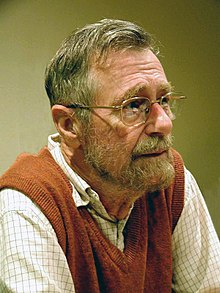
\includegraphics[width=0.2\textwidth]{dijkstra}
\caption{Edsger Wybe \dijkstra}\label{fig:dijkstra}
\end{figure}

\section{Théorie des Graphes}
\subsection{Introduction}
La théorie des graphes s'est développée au cours du \textsc{XX}\ieme siécle.
La génèse de la théorie des graphes semble être une étude de Léonard
\nom{Euler}, un très célèbre mathématicien du \textsc{XVIII}\ieme.
Dans un article publié en 1736, il traite un problème devenu classique,
illustré par la devinette : peut on faire une promenade passant une fois par
chacun des sept ponts de la ville de Koenigsberg?
Regardez la figure~\ref{fig.koenig}.
\begin{figure}
\centering
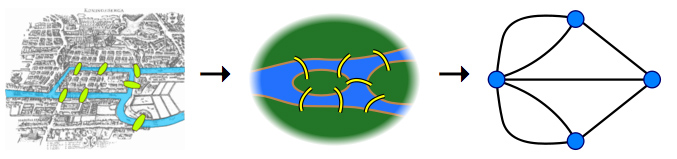
\includegraphics[width=0.8\textwidth]{koenigsberg}
\caption{Koenigsberg}\label{fig.koenig}
\end{figure}
\subsection{Les bases pour comprendre \algo}

\begin{defi}
  Un graphe $\Gamma(S, A)$ est la donnée de deux ensembles finis: un ensemble de
  sommets $S$ et un ensemble d’arêtes $A$. Une arête est une paire de sommets,
  ce sont les extrémités de l’arête. Une arête $\Set{x, y}$ est notée $xy$,
  et les sommets sont dits adjacents.
\end{defi}
\begin{defi}
  Un chemin de longueur n est une suite de  sommets $x_0, x_1, \dots , x_n$
  tels que :
  \[
  \forall i,\, 0 \leq i < n \implies x_i, x_{i+1} \in A
  \]
  Les sommets $x_0$ et $x_n$ sont les extrémités du chemin, $x_0$ est l’origine
et $x_n$ le sommet terminal. On parle de cycle quand $x_0 = x_n$. On dit
que $x$ est connecté à $y$, et on note $x \to y$ quand il existe un chemin
d’extrémité x et y. Il s’agit là d’une relation symétrique et transitive
qu’il convient de prolonger par réflexivité. Un chemin est dit simple
quand il ne passe jamais plus d’une fois par une même arête. Un chemin
élémentaire ne passe pas deux fois par un même sommet.
\end{defi}
\begin{defi}
L’ensemble des sommets voisins d’un sommet $x$ :
\[
\text{voisin($x$)} = \Set{ y \in S | xy \in A },\quad \text{deg($x$) = $\#$voisin($x$)}
\]
le degré d’un sommet est égal au nombre d’arêtes incidentes. Un
sommet de degré pair est dit pair, un sommet de degré impair est
dit impair.
\end{defi}
Nous avons l’amusante relation des paires et de l’impair
\begin{lemme}
  (parité et impairs). Dans un graphe, $\Gamma(S, A)$ :
  \[
  \sum_{x \in S} \text{deg($x$)} = 2 \lvert A \rvert
  \]
  en particulier, le nombre des sommets impairs est toujours pair.
\end{lemme}
\begin{proof}
  Notons $A_s$ les arêtes incidentes au sommet $s$,
  \[
  A = \bigcup_{s \in S} A(s).
  \]
Une triple intersection des $A_s$ est vide, une double intersection non
vide est une arête du graphe. Le principe d’inclusion et d’exclusion  s’applique sans difficulté et donne :
\[
\lvert A \rvert = \sum_{s \in S} \text{deg($s$)} - \lvert A \rvert
\]
\end{proof}
\begin{exo}
Prouver qu’un graphe d’ordre supérieur à 1, possède deux sommets de degré identique.
\end{exo}
\begin{exo}
 De tout parcours, on peut extraire un parcours élémentaire
ayant les mêmes extrémités. Détaillez cette affirmation !
\end{exo}
\begin{exo}
 Dans un graphe acyclique ayant au moins une arête, il existe un sommet de degré 1. Expliquez !
\end{exo}
Pour creuser plus sur l'intéresant théorie des graphes~\cite{langevin.book}.

\section{L'\algo}
\subsection{Le principe}
L'algorithme prend en entrée un graphe pondéré par des réels positifs et un sommet source. Il s'agit de construire progressivement un sous-graphe dans lequel sont classés les différents sommets par ordre croissant de leur distance minimale au sommet de départ. La distance correspond à la somme des poids des arcs empruntés.

Au départ, on considère que les distances de chaque sommet au sommet de départ sont infinies, sauf pour le sommet de départ pour lequel la distance est nulle. Le sous-graphe de départ est l'ensemble vide.

Au cours de chaque itération, on choisit en dehors du sous-graphe un sommet de distance minimale et on l'ajoute au sous-graphe. Ensuite, on met à jour les distances des sommets voisins de celui ajouté. La mise à jour s'opère comme suit : la nouvelle distance du sommet voisin est le minimum entre la distance existante et celle obtenue en ajoutant le poids de l'arc entre sommet voisin et sommet ajouté à la distance du sommet ajouté.
On continue ainsi jusqu'à épuisement des sommets (ou jusqu'à sélection du sommet d'arrivée).
\subsection{Schéma de l'algorithme}
Le graphe est noté  $G=(S,A)$ où :
\begin{itemize}
\item l'ensemble $S$ est l'ensemble fini des sommets du graphe $G$ ;
\item l'ensemble $A$ est l'ensemble des arcs de $G$ tel que : si $(s_{1},s_{2})$ est dans $A$, alors il existe un arc depuis le nœud $s_{1}$ vers le nœud $s_{2}$ ;

\item on définit la fonction \emph{poids} définie sur $S \times S$ dans $ \R^{+}\cup \{+\infty \}$ qui à un couple $(s_{1},s_{2})$ associe le poids positif \emph{$poids(s_{1},s_{2})$}  de l'arc reliant $s_{1}$ à $s_{2}$ (et $+\infty$ s'il n'y a pas d'arc reliant $s_{1}$ à $s_{2}$).
\end{itemize}
Le poids du chemin entre deux sommets est la somme des poids des arcs qui le composent. Pour une paire donnée de sommets $s_{deb}$ (le sommet du départ) $s_{fin}$ (le sommet d'arrivée) appartenant à $S$, l'algorithme trouve un chemin depuis $s_{deb}$ vers $s_{fin}$ de moindre poids (autrement dit un chemin le plus léger ou encore le plus court).

L'algorithme fonctionne en construisant un sous-graphe $P$ de manière que la distance entre un sommet $s$  de $P$ depuis $s_{deb}$ soit connue et soit un minimum dans $G$. Initialement, $P$ contient simplement le nœud $s_{deb}$ isolé, et la distance de $s_{deb}$ à lui-même vaut zéro. Des arcs sont ajoutés à $P$ à chaque étape :
\begin{enumerate}
\item en identifiant tous les arcs $a_{i}=(s_{i1},s_{i2})$ dans $P\times G$;
\item en choisissant l'arc $a_{j}=(s_{j1},s_{j2})$ dans $P\times G$ qui donne la distance minimum depuis $S_{deb}$  à $s_{j2}$ en passant tous les chemins créés menant à ce nœud.
\end{enumerate}
L'algorithme se termine soit quand $P$ devient un arbre couvrant de $G$, soit quand tous les nœuds d'intérêt sont dans $P$.
Information tiré de~\cite{dijkstra.algo.wiki}.
\subsection{L'\algo en C++}
On voit à la figure~\ref{algo_code} une implementation du code en C++
\begin{figure}[!htb]
\lstinputlisting[
    language=C++,
    style=myStyle,
]{dijkstra.cpp}
\caption{L'\algo en C++}\label{algo_code}
\end{figure}

\subsection{Exemple graphique}
\begin{figure}[!htb]
\centering
\begin{tikzpicture}[node distance={25mm}, thick, main/.style = {draw, circle}]
\node[main] (1) {A};
\node[main] (2) [right of=1] {B};
\node[main] (3) [below right of=1] {C};
\node[main] (4) [below right of=2] {D};
\node[main] (5) [right of=2] {E};

\draw (1) -- node[midway, above, pos=0.5] {3} (2);
\draw (1) -- node[midway, above, sloped, pos=0.5] {1} (3);
\draw (2) -- node[midway, above, sloped, pos=0.5] {7} (3);
\draw (3) -- node[midway, above , pos=0.5] {2} (4);
\draw (2) -- node[midway, above, sloped, pos=0.5] {5} (4);
\draw (2) -- node[midway, above , pos=0.5] {1} (5);
\draw (4) -- node[midway, above, sloped, pos=0.5] {7} (5);
\end{tikzpicture}
\caption{Graphe d'exemple}
\label{graphbase}
\end{figure}
Supposons le graphe pondéré de la figure~\ref{graphbase}.

Pendant l'exécution de l'algorithme, nous allons marquer chaque nœud avec sa
distance minimale au nœud C (notre nœud sélectionné). Pour le noeud C, cette
distance est 0. Pour le reste des noeuds, comme nous ne connaissons pas encore
cette distance minimale, elle commence à l'infinie ($\infty$).
Nous aurons également un noeud courant. Initialement, nous le définissons sur C
(notre nœud sélectionné). Dans l'image, nous marquons le nœud actuel avec un
point rouge. Regardez la figure~\ref{fig:all_inf}.

\begin{figure}[!htb]
\centering
\begin{tikzpicture}[node distance={25mm}, thick, main/.style = {draw, circle}]
\node[main, label=above:{$\infty$}] (1) {A};
\node[main, label=above:{$\infty$}] (2) [right of=1] {B};
\node[main, label=below:{$\textcolor{red}{\bullet} 0$}] (3) [below right of=1] {C};
\node[main, label=below:{$\infty$}] (4) [below right of=2] {D};
\node[main, label=above:{$\infty$}] (5) [right of=2] {E};
\draw (1) -- node[midway, above, pos=0.5] {3} (2);
\draw (1) -- node[midway, above, sloped, pos=0.5] {1} (3);
\draw (2) -- node[midway, above, sloped, pos=0.5] {7} (3);
\draw (3) -- node[midway, above , pos=0.5] {2} (4);
\draw (2) -- node[midway, above, sloped, pos=0.5] {5} (4);
\draw (2) -- node[midway, above , pos=0.5] {1} (5);
\draw (4) -- node[midway, above, sloped, pos=0.5] {7} (5);
\end{tikzpicture}
\caption{Etape 1}\label{fig:all_inf}
\end{figure}

Maintenant, vérifions les voisins de notre nœud actuel (A, B et D) sans ordre particulier. Commençons par B. Nous ajoutons la distance minimale du nœud actuel (dans ce cas, 0) au poids de l'arête qui relie notre nœud actuel à B (dans ce cas, 7), et nous obtenons 0 + 7 = 7. Nous comparons cette valeur avec la distance minimale de B (infini); la valeur la plus petie est celle qui reste comme distance minimale de B (dans ce cas, 7 est plus pétit que l'infini) et ainsi de suite pour les autres voisins.

Nous avons vérifié tous les voisins de C. Pour cette raison, on le marque comme visité.

Nous devons maintenant choisir un nouveau noeud courant. Ce noeud doit être le noeud non visité avec la plus petite distance minimale (donc, le noeud avec le plus petit nombre et sans marque de contrôle). C'est A. Marquons-le d'un point rouge. Regardez la figure~\ref{fig:etp_2}.
\begin{figure}[!htb]
\centering
\begin{tikzpicture}[node distance={25mm}, thick, main/.style = {draw, circle}]
\node[main, label=above:{$\textcolor{red}{\bullet}1$}] (1) {A};
\node[main, label=above:{$7$}] (2) [right of=1] {B};
\node[main, label=below:{$\textcolor{green}{\checkmark} 0$}] (3) [below right of=1] {C};
\node[main, label=below:{$2$}] (4) [below right of=2] {D};
\node[main, label=above:{$\infty$}] (5) [right of=2] {E};
\draw (1) -- node[midway, above, pos=0.5] {3} (2);
\draw (1) -- node[midway, above, sloped, pos=0.5] {1} (3);
\draw (2) -- node[midway, above, sloped, pos=0.5] {7} (3);
\draw (3) -- node[midway, above , pos=0.5] {2} (4);
\draw (2) -- node[midway, above, sloped, pos=0.5] {5} (4);
\draw (2) -- node[midway, above , pos=0.5] {1} (5);
\draw (4) -- node[midway, above, sloped, pos=0.5] {7} (5);
\end{tikzpicture}
\caption{Etape 2}\label{fig:etp_2}
\end{figure}

Et maintenant nous répétons l'algorithme. Nous vérifions les voisins de notre nœud actuel, en ignorant les nœuds visités. Cela signifie que nous ne vérifions que B.

Pour B, nous ajoutons 1 (la distance minimale de A, notre noeud actuel) à 3 (le poids de l'arête reliant A et B) pour obtenir 4. Nous comparons ce 4 avec la distance minimale de B (7) et nous laissons la plus petite valeur : 4. Regardez la figure~\ref{fig:etp_3}.

\begin{figure}[!htb]
\centering
\begin{tikzpicture}[node distance={25mm}, thick, main/.style = {draw, circle}]
\node[main, label=above:{$\textcolor{red}{\bullet}1$}] (1) {A};
\node[main, label=above:{$4$}] (2) [right of=1] {B};
\node[main, label=below:{$\textcolor{green}{\checkmark} 0$}] (3) [below right of=1] {C};
\node[main, label=below:{$2$}] (4) [below right of=2] {D};
\node[main, label=above:{$\infty$}] (5) [right of=2] {E};
\draw (1) -- node[midway, above, pos=0.5] {3} (2);
\draw (1) -- node[midway, above, sloped, pos=0.5] {1} (3);
\draw (2) -- node[midway, above, sloped, pos=0.5] {7} (3);
\draw (3) -- node[midway, above , pos=0.5] {2} (4);
\draw (2) -- node[midway, above, sloped, pos=0.5] {5} (4);
\draw (2) -- node[midway, above , pos=0.5] {1} (5);
\draw (4) -- node[midway, above, sloped, pos=0.5] {7} (5);
\end{tikzpicture}
\caption{Etape 3}\label{fig:etp_3}
\end{figure}

Ensuite, nous marquons A comme visité et choisissons un nouveau noeud courant :
D, qui est le nœud non visité avec la plus petite distance actuelle.
Regardez la figure~\ref{fig:etp_4}.
\begin{figure}[!htb]
\centering
\begin{tikzpicture}[node distance={25mm}, thick, main/.style = {draw, circle}]
\node[main, label=above:{$\textcolor{green}{\checkmark}1$}] (1) {A};
\node[main, label=above:{$4$}] (2) [right of=1] {B};
\node[main, label=below:{$\textcolor{green}{\checkmark} 0$}] (3) [below right of=1] {C};
\node[main, label=below:{$\textcolor{red}{\bullet}2$}] (4) [below right of=2] {D};
\node[main, label=above:{$\infty$}] (5) [right of=2] {E};
\draw (1) -- node[midway, above, pos=0.5] {3} (2);
\draw (1) -- node[midway, above, sloped, pos=0.5] {1} (3);
\draw (2) -- node[midway, above, sloped, pos=0.5] {7} (3);
\draw (3) -- node[midway, above , pos=0.5] {2} (4);
\draw (2) -- node[midway, above, sloped, pos=0.5] {5} (4);
\draw (2) -- node[midway, above , pos=0.5] {1} (5);
\draw (4) -- node[midway, above, sloped, pos=0.5] {7} (5);
\end{tikzpicture}
\caption{Etape 4}\label{fig:etp_4}
\end{figure}
Nous répétons à nouveau l'algorithme. Cette fois, nous vérifions B et E.

Pour B, nous obtenons 2 + 5 = 7. Nous comparons cette valeur avec la distance minimale de B (4) et laissons la plus petite valeur (4). Pour E, nous obtenons 2 + 7 = 9, nous la comparons avec la distance minimale de E (infini) et nous laissons la plus petite (9).

Nous marquons D comme visité et mettons notre noeud actuel à B.
Regardez la figure~\ref{fig:etp_5}.
\begin{figure}[!htb]
\centering
\begin{tikzpicture}[node distance={22mm}, thick, main/.style = {draw, circle}]
\node[main, label=above:{$\textcolor{green}{\checkmark}1$}] (1) {A};
\node[main, label=above:{$4$}] (2) [right of=1] {B};
\node[main, label=below:{$\textcolor{green}{\checkmark} 0$}] (3) [below right of=1] {C};
\node[main, label=below:{$\textcolor{green}{\checkmark}2$}] (4) [below right of=2] {D};
\node[main, label=above:{$9$}] (5) [right of=2] {E};
\draw (1) -- node[midway, above, pos=0.5] {3} (2);
\draw (1) -- node[midway, above, sloped, pos=0.5] {1} (3);
\draw (2) -- node[midway, above, sloped, pos=0.5] {7} (3);
\draw (3) -- node[midway, above , pos=0.5] {2} (4);
\draw (2) -- node[midway, above, sloped, pos=0.5] {5} (4);
\draw (2) -- node[midway, above , pos=0.5] {1} (5);
\draw (4) -- node[midway, above, sloped, pos=0.5] {7} (5);
\end{tikzpicture}
\caption{Etape 5}\label{fig:etp_5}
\end{figure}

Nous répétons l'algorithme pour chaque noeud et à la fin nous obtenons le graphe
de  la figure~\ref{fig:final_graph}.
\begin{figure}[!htb]
\centering
\begin{tikzpicture}[node distance={25mm}, thick, main/.style = {draw, circle}]
\node[main, label=above:{$\textcolor{green}{\checkmark}1$}] (1) {A};
\node[main, label=above:{$\textcolor{green}{\checkmark}4$}] (2) [right of=1] {B};
\node[main, label=below:{$\textcolor{green}{\checkmark}0$}] (3) [below right of=1] {C};
\node[main, label=below:{$\textcolor{green}{\checkmark}2$}] (4) [below right of=2] {D};
\node[main, label=above:{$\textcolor{green}{\checkmark}5$}] (5) [right of=2] {E};
\draw (1) -- node[midway, above, pos=0.5] {3} (2);
\draw (1) -- node[midway, above, sloped, pos=0.5] {1} (3);
\draw (2) -- node[midway, above, sloped, pos=0.5] {7} (3);
\draw (3) -- node[midway, above , pos=0.5] {2} (4);
\draw (2) -- node[midway, above, sloped, pos=0.5] {5} (4);
\draw (2) -- node[midway, above , pos=0.5] {1} (5);
\draw (4) -- node[midway, above, sloped, pos=0.5] {7} (5);
\end{tikzpicture}
\caption{Graphe finale}\label{fig:final_graph}
\end{figure}
Pour plus d'information~\cite{example.web}.

\section{Complexité}
\subsection{Rappels sur la complexité}
\begin{defi}
   Soit $g$ une fonction de $\mathfrak{F}$. On définit respectivement les notations grand omicron et grand oméga:
   \[
   O(g) := \Set{f \in \mathfrak{F} | \exists c>0\quad \exists N \in \ensemble{N}\quad
     \forall n \geq N \quad 0 \leq f(n) \leq cg(n)}
   \]
   \[
   \Omega(g) := \Set{f \in \mathfrak{F} | \exists c>0\quad \exists N \in \ensemble{N}\quad
     \forall n \geq N \quad 0 \leq cg(n) \leq  f(n) }
   \]
\end{defi}
\begin{defi}
   Soit $g$ une fonction de $\mathfrak{F}$. On définit la notation grand thêta:
   \[
   \Theta(g) := \Set{f \in \mathfrak{F} |\exists a>0 \quad \exists b>0\quad \exists N \in \ensemble{N}\quad
     \forall n \geq N \quad 0 \leq ag(n) \leq  f(n) \leq bg(n) }
   \]
\end{defi}
\begin{prop}
  Soient $f$ et $g$ deux fonctions de $\mathfrak{F}$. On a
  \[
  f = \Theta(g) \iff f = O(g) \quad \text{et} \quad f = \Omega(g)
  \]
\end{prop}
L'expression algébrique d'une fonction et quelques connaissances sur la croissance des fonctions réelles suffisent parfois à mettre en évidence qu'une majoration est grossière, par exemple quand on affirme que la fonction $n\to 2n+1$ est en $O(n^3)$.
Ce n'est pas la définition de la notation $O$ qui nous permet d'affirmer que cette estimation est grossière mais la connaissance de la croissance des fonctions monomiales.
Ainsi l'écriture $f=O(g)$ ne précise pas si $f$ croit beaucoup moins vite que toute constante fois $g$ asymptotiquement ou si $f$ s'en approche.
La notation petit $o$ répond partiellement à cette question, quand on écrit$f=o(g)$,
on signifie que:
\[
\lim_{n \to + \infty}\frac{f(n)}{g(n)} = 0
\]
\begin{defi}
  Soit $g$ une fonction de $\mathfrak{F}$. On définit respectivement les
  notations petit omicron et petit oméga:
   \[
   o(g) := \Set{f \in \mathfrak{F} | \forall c>0\quad \exists N \in \ensemble{N}\quad
     \forall n \geq N \quad 0 \leq f(n) \leq cg(n)}
   \]
   \[
   \omega(g) := \Set{f \in \mathfrak{F} | \forall c>0\quad \exists N \in \ensemble{N}\quad
     \forall n \geq N \quad 0 \leq cg(n) \leq  f(n) }
   \]
\end{defi}
Pour plus d'information sur la théorie de l'infomation~\cite{zanotti.complex}
\subsubsection{Estimation de l'efficacité}
En calculant la complexité en temps d'un algorithme, il est possible de vérifier, avant de le mettre en œuvre, si'il est suffisamment efficace pour le problème. Nous partons pour les estimations qu'un ordinateur moderne peut effectuer quelques centaines de millions d'opérations en une seconde.

Par exemple, supposons que le temps limite pour un problème est d'une seconde et que la taille de l'entrée est $n = 10^{5}$.  Si la complexité est $O(n^{2})$, l'algorithme effectuera environ ${(10^{5})}^2 = 10^{10}$ operations.
Cela devrait prendre au moins quelques dizaines de secondes. Donc l'algorithme semble donc trop lent pour résoudre le problème.
D'un autre côté, étant donné la taille de l'entrée, nous pouvons essayer de deviner la complexité requise pour l'algorithme.
Le tableau \ref{fig:time_tab} contient quelques estimations utiles en supposant une limite de temps d'une seconde.
Informations utiles sur la complexité~\cite[p.~20]{comp.prog.book}.
\begin{figure}
  \[
  \begin{array}{|c|c|}
    \hline
    \text{taille de l'entrée} & \text{complexité requise} \\
    \hline
    n \leq 10 & O(n!) \\
    \hline
    n \leq 20 & O(2^n) \\
    \hline
    n \leq 500 & O(n^3) \\
    \hline
    n \leq 5000 & O(n^2) \\
    \hline
    n \leq {10}^6 & O(nlog(n)) \quad \text{ou} \quad O(n) \\
    \hline
    n > {10^6} & O(1)\quad \text{ou} \quad O(log(n)) \\
    \hline
  \end{array}
  \]
  \caption{Temps d'execution par taille de l'entrée}\label{fig:time_tab}
\end{figure}
\subsection{Complexité de l'\algo}
L'efficacité de l'algorithme de Dijkstra repose sur une mise en œuvre efficace
de la recherche du minimum. L'ensemble $\mathcal{Q}$ est implémenté par une
file à priorités. Si le graphe possède $\lvert A \rvert$ arêtes et $\lvert S \rvert$
sommets, qu'il est représenté par des listes d'adjacence et si on implémente
la file à priorités par un tas binaire (en supposant que les comparaisons des
poids des arêtes soient en temps constant), alors la complexité en temps de
l'algorithme est $O((\lvert A \rvert + \lvert S \rvert)\times \log(\lvert S \rvert))$.
En revanche, si on implémente la file à priorités avec un tas de Fibonacci,
l'algorithme est en $O(\lvert A \rvert + \lvert S \rvert \times \log(\lvert S \rvert))$.


\section{Applications}
L'\algo est appliqué pour le calcul d'itinéraires routiers
comme sur les sites Web de cartographie comme \textit{MapQuest} ou
\textit{Google Maps}.
Le poids des arcs pouvant être la distance (pour le trajet le plus court),
le temps estimé (pour le trajet le plus rapide), la consommation de carburant
et le prix des péages (pour le trajet le plus économique).

Une application courante de l'algorithme de Dijkstra apparaît dans les
protocoles de routage interne \glms{à état de liens}, tels que
\textit{Open Shortest Path First} ou encore \textit{PNNI} sur les réseaux
\textit{ATM}, qui permettent un routage internet très efficace des
informations en cherchant le parcours le plus efficace.

\bibliographystyle{plain}
\bibliography{biblio}

\end{document}
